\section{Discussion and Future Work}

We now reflect on broader issues and opportunities that arose during the development and evaluation of \toolname{}.

\begin{figure*}[!h]
    \centering
    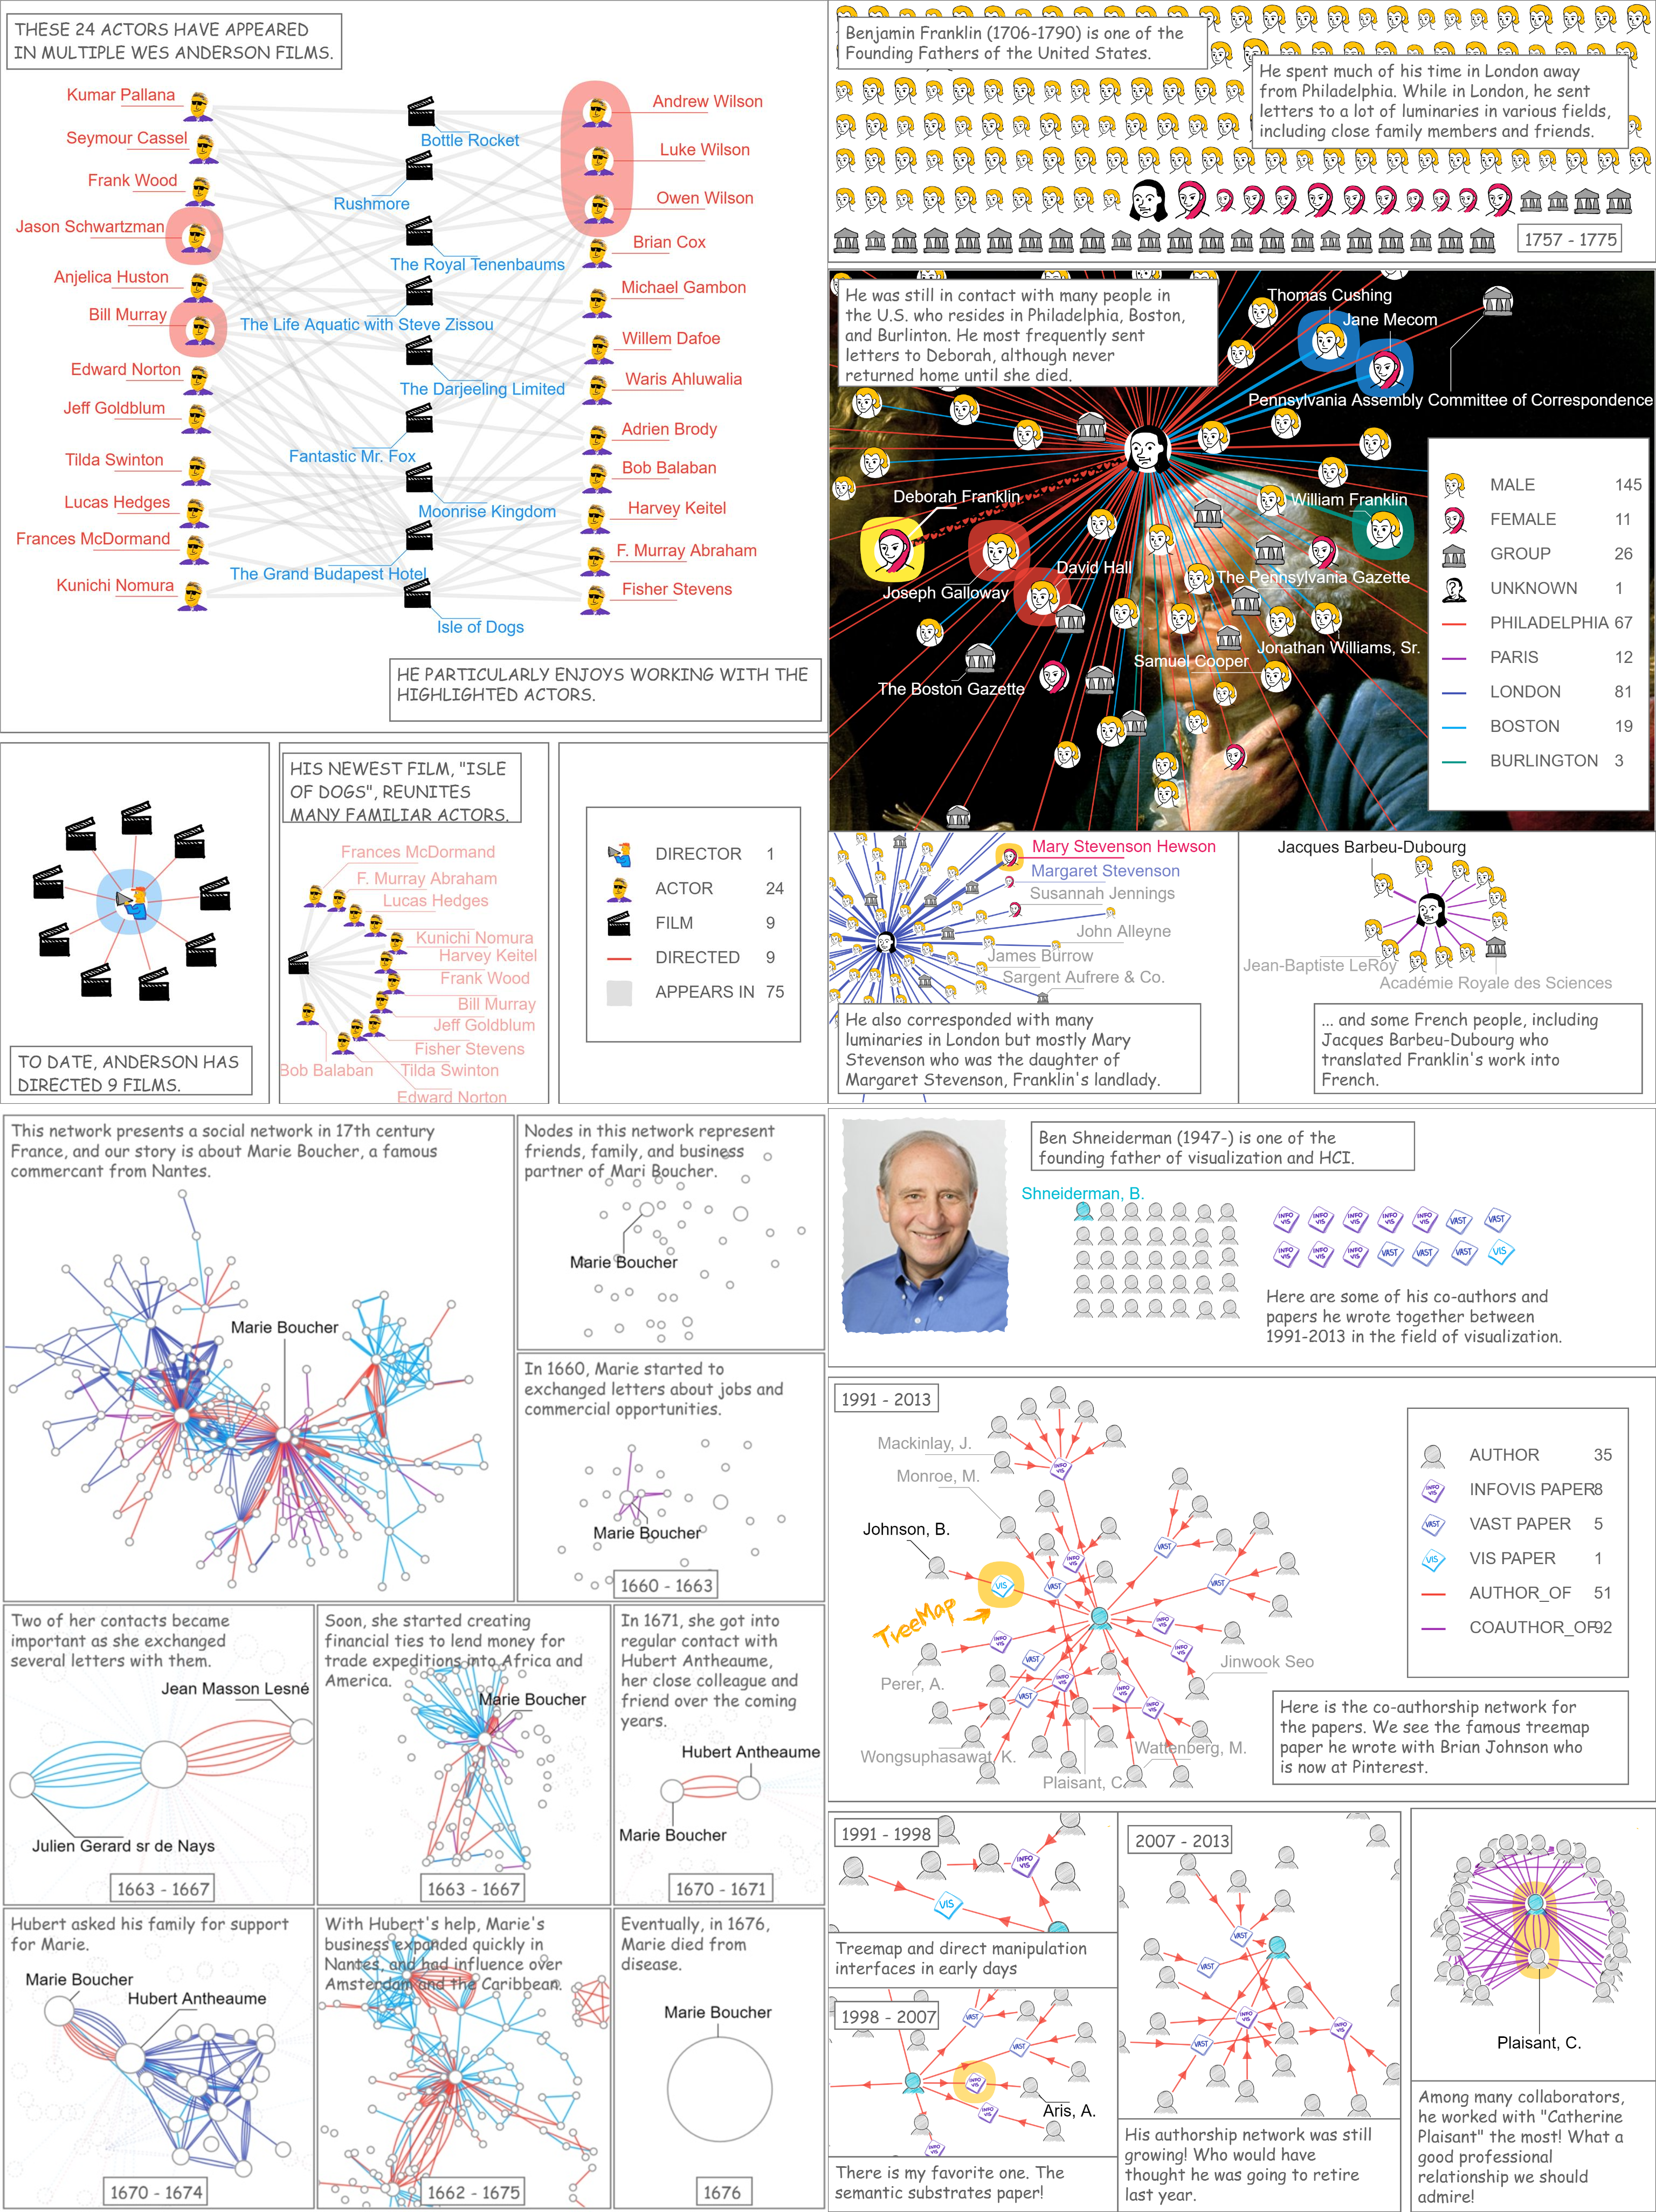
\includegraphics[width=1.0\textwidth]{figures/examples.jpeg}
    % 
\includegraphics[width=1.0\textwidth]{figures/examples-new.png}
    \caption{A gallery of eight data comics created with \toolname{} using different \rev{comic styles} and datasets.}
	\label{fig:examples}
    %  \vspace{-0.2cm}
\end{figure*}

\vspace{2mm}
% \bpstart{Beyond dynamic networks}

\bpstart{Generalization to other data and visualization types} \rev{The design of \toolname{} (See \autoref{fig:interaction}) is mostly data-type-agnostic and generalizable beyond network data, such as gestures, panel manipulation, annotations, time sliders, highlighting and removing data elements, etc. Accommodating other data types (e.g., tabular data), visualizations (e.g., bar charts), and specific components (e.g., axes and scales) is an interesting research direction. The overarching research question in this space would be how to enable fast and fluid creation and manipulation of such panels, as visualizations can involve complex grouping and filtering operations on data. However, core ``comic'' features such as automatic propagation of style, automatic generation of transitions and panel recommendation would require minimum redesign.}


% While \toolname{} was designed for creating comics about dynamic networks, adding the ability to import other forms of data, such as tabular data, may increase its appeal. Support for other forms of data would also necessitate visualization types beyond node-link diagrams and unit charts, which would in turn increase the tool's expressiveness. Matrices and other visualization types used for dynamic networks are also worth considering.
% However, it is likely that our current interactions may require adjustment to accommodate new visualization types; for instance, lassoing as a selection interaction is unlikely to be compatible with a matrix visualization.

%\nam{not sure what is being discussed here:}it can already been used to show other data such as timelines (Fig. XX), trajectories (Fig. XX), or simply quantities (Fig. XX). However, 


% the general concept and interaction design of DataToon can be adapted to other types of data (e.g. time-series, charts). Supporting different types of datasets such as tables as well as other common visualization types such as bar charts and line charts would further increase DataToon's expressivity and usefulness. 

% Most of our design choices can generalize to other data and visualization types, though some adjustments to our interactions may be required to accommodate them (e.g., free-form lassoing is unlikely to be effective in the context of matrix diagrams). Though perhaps the most obvious next step in extending DataToon involves adding automatic geo-encoding so that the author no longer needs to manually position nodes on images of maps, as in \autoref{fig:workflow}. Our transition feature is likely to be particularly useful for any data that changes over time, as a first step toward automatically generating panels, helping authors to lay out their story.
%\nam{maybe it's worthwhile to expand the discussion of this:}
\vspace{2mm}
\bpstart{Pen + touch interaction for data-driven storytelling} Pen + touch interaction was seen as engaging and flexible by our study participants, advantages that may prove beneficial beyond data comics to other data-driven storytelling experiences. While novices require time to acclimate to pen + touch interfaces, we observed that after an initial learning phase, this input modality stimulates creativity and encourages experimentation. However, to promote learning and discoverability, we must design appropriate visual cues and affordances that remind users of their capabilities. In our study, we observed that people initially want to use pen and touch interchangeably to accomplish a single action. This observation warrants further investigation and a revisitation of the {\it pen writes, touch manipulates} mantra~\cite{hinckley2010pen}.

%To ensure that DataToon for those without pen and touch devices, we are also currently developing a browser-based version that supports conventional mouse and keyboard input. %Ben: of course we do not, but I feel it'd be nice to think about it for wide usage.
% \nam{Can we say more directly about the limitations and lessons we learned to better inform future research? Here is what I wrote before. It is not streamlined but I find the above discussion too generic somehow:}
%Considering our study findings along with our own experience of creating data comics (\autoref{fig:examples}, we identified several ways to further improve DataToon. A common issue associated with any gesture-based tool is that it is difficult to determine which operations are possible upon initial use. 
%As we observed in our study, one might be initially unsure as to which (pen or touch) gestures are required to execute on the various visual elements. This issue is exacerbated by the fact that many of these elements comprise parts of visualization. The abstract forms of elements within a visualization lack the natural affordances of physical objects. It could be useful to identify visual cues provide hints with respect to interaction modality, reducing the gulf of execution. Since people are used to manipulating objects via touch, it would be useful to investigate how manipulation via touch differs from a pen. 

%When it comes to authoring a data comic, one must manipulate many visualization elements. Most existing visualization tools that make use of multi-touch interaction for manipulating objects operate at the visualization level, and there is no established vocabulary for interacting with visualization content, which usually consists of many small marks. Our decision to include multiple pen tools is still suboptimal as it often requires many mode switchings (e.g., creating a node label and positioning nodes). Instead of mode switching, an alternative approach would be to devise an intelligent mechanism to detect a author's intention. For example, when an author holds a panel, we can infer that she is trying to manipulate its content, implicitly switching the pen type from a regular pencil to a control annotation pen. 

% Additional issues arise when polishing the comic to create a final version for presentation. Although the flexibility of storyboarding in \toolname{} enabled rapid exploration of design alternatives, it lacks some precise control in aligning panels for example. Thus, in the future we plan on providing an intelligent snapping of panels while taking into account the gutters between them. Additional features related to polishing a data comics include possibilities to turn handwriting to text, and beautified versions of sketched elements. 

\vspace{2mm}
\bpstart{Beyond traditional comics}
\toolname{} exports pages as static images, like traditional comic books. While being respectful of this tradition, creating dynamic and interactive data comics is an interesting research direction. For example, a ``presentation mode'' might allow for presenters or viewers to touch parts of the comic and reveal content on demand, or add annotations as part of an active reading process~\cite{walny2018active}. Alternatively, \toolname{} could export comics as websites that invite viewer interaction, potentially by integrating techniques such as brushing and linking across panels.

% \bstart{Additional Features}
% During the design, development, and evaluation of DataToon, we found many features that are straightforward to add which would further improve the workflow. Examples include support for panel layout and further templates (for examples see ~\cite{bachdesign}), sizing and alignment, guiding the manual labor without reducing expressiveness. 
% While our transitions are currently limited to \nam{we acutually have more, filter build up, zoom transform, panel sizes.} temporal sequences, we can easily imagine creating multi-panel transitions for pan and zoom or complex processes such as changes to clusters,described elsewhere~\cite{bach2016telling}.
% \matt{this paragraph is redundant, and nam says multiple transitions are supported, rendering the final part of it moot}
% \vspace{.1cm}
\vspace{2mm}
\bpstart{Toward higher-level narrative design support} Our design considerations emphasized use of the structural elements of comics such as panels and captions to convey a data story. However, producing an engaging story still depends on the contents of the data and the creativity of the author. \toolname{} does not explicitly incorporate higher-level narrative design patterns~\cite{bachdesign,bach2018napa} into its interface. 

The automatic transition, suggestion, and layout template features are a step toward narrative design guidance, but there are further opportunities to improve
% , but further study and design iteration are required to determine if we have satisfied our fourth design consideration
. For example, we might auto-populate an entire template with visualization content as a way to seed a story, though we must take care to not absolve authors of their creative agency. Similarly, generating panel transitions that precisely match an author's narrative intent is challenging, but such transitions can be used as a way discover new narrative directions. Also, being able to quickly evaluate the overall narrative structure will greatly aid the iterative process of crating a story~\cite{storycurve}.



%For these kinds of narration support, we could draw inspirations from the established field of computational narrative as well.




% \toolname{}'s layout templates are currently initialized with empty panels. It would be an interesting challenge to partially or entirely fill these panels automatically as a way to seed a story. As with transitions, we imagine that it is unreasonable to automate the generation of narrative structure in way that precisely mirrors the author's intent. Thus, a mixed initiative approach could be a viable solution. 



% With DataToon, we tried to find the middle ground between an unconstrained yet unspecific graphic authoring tool and a visualization-specific authoring environment. Our solution thereby allows for considerable expressiveness in terms of panel layout and node styling. These features borrow from the features available in many graphics editing tools such as Adobe Illustrator. Our examples in \autoref{fig:examples} show that DataToon allows for the realization of most of the design patterns for data comics described by Bach et al.~\cite{bachdesign}, including ``time-sequence'' and ``the-larger-picture''. 


% Eventually, we are interested in investigating higher-level narrative structures that help authors to produce long-form multi-page stories with a beginning, middle, and end.

% including a proper beginning, middle, and end, or non-linear storytelling~\cite{storycurve}. 
% \matt{I don't see how this isn't possible now. mentioning Story curves is a distracting non-sequitor.}
% It remains to be seen which features of DataToon will find useful during their work. 


% Our transition feature is likely to be particularly useful for any data that changes over time, as a first step toward automatically generating panels, helping authors to lay out their story.

% \toolname{} currently focuses on creating structural elements of data comics (visualizations, panels, etc), as opposed to semantic elements such as narrative design patterns.



% For example, while an author can draw a path between two panels to generate transitions between then, we could similarly attempt to predict future panels an existing panel or an existing transition, thereby recommending panels to authors.

% \nam{Another part I wrote before. I thought it would be nice to expand the discussion of ``Working with Data'' above in more detail.}
% \vspace{.1cm}
% \vspace{2mm}
% \bpstart{Beyond reproduction}
% \nam{I think this subsection can be cut, or reduced and moved to conclusion as a future work.}
% Our study results suggest that \toolname{} is easy to learn and that people without expertise in graphic design can create data comics using it. 

% We plan to extend our evaluation to study the authoring process in a more longitudinal {\it free-form study}~\cite{ren2018beliv}, in which participants create comics with their own data in their own workspace, as opposed to reproducing them in lab settings.  Such a study could provide additional evidence for \toolname{}'s expressiveness, as well its efficiency and compatibility with authors' existing workflows, both being criteria of interest when evaluating visualization authoring tools~\cite{amini2018}.
% By understanding the differences in the processes, we hope to uncover insights for further improving the tool. 
% In addition to creating a story, being able to evaluate the story would also be important~\cite{storycurve}. 

% We originally developed DataToon to be used specifically for authoring data comics to communicate known insights.





% \rev{The advanced features including the transition and automatic suggestions are not rigorously evaluated. In what manner do they facilitate data exploration and authoring a visual data story? We focused on the authoring, what about reading experiences or evaluating the story using story curves. }



% Combining exploration in the presentation side.

% In this work, we have only scratched the surface in terms of the design space of authoring tools for data comics. We see several opportunities to further leverage the underlying data in the design of future authoring tools.  




% \nam{Work in progress, please feel free to chime in...}
% 2. Transferring and sharing contents across the pages. Interactive data comics, nonlinear reading experiences through coordinated panels.
% \matt{Not substantive}

% The benefit of having access to the underlying data may also be useful in a live presentation context, or in a context that allows for limited exploration, such as in an interactive museum or gallery exhibit.



% Our observation in the user study showed that people used the tool to explore data. The ability to freely annotate and manage multiple panels provide a form of active reading capability~\cite{walny2018active}..

%%BEN: I left the previous text below and tried to integrate as much of the information into the new version. The full old version is at --discussion.tex--

% \section{Discussion}

% \subsection{Limitations and opportunities for further improvements}
% \nam{reduce}
% The result of the user study, as well as our own experience of creating examples of data comics (\autoref{fig:examples}, illuminated further possible improvements of our tool. A common issue associated with any gesture-based tool is that it is difficult to figure out what operations are possible in the first place. As we observed in the user study, it could be initially confusing to users what gestures (pen or touch) are required to execute on which types of visual elements. This issue becomes more challenging when a visualization is the main content. The abstract form of the visualization lack natural affordances available in physical objects. It could be useful to come up with visual cues that can hint on available interaction modality, reducing the gulf of execution. Since people are used to using touch to manipulate objects, it would be useful to investigate in which parts touch feels more natural than the pen. 

% When it comes to creating a data comic, it requires an author to manipulate on fine-grained elements of the visualization (e.g., selecting and annotating a small set of elements). Most existing visualization tools employing multi-touch interaction for manipulating context operate at the visualization level. There is no established vocabulary for interacting the visualization content which usually consists of a  lot of small data points. Our decision to have multiple pen tools instead of fingers is still suboptimal as it often requires a significant number of mode switchings (e.g., creating a node label and positioning the node. Instead of requiring the mode switching, devising an intelligent mechanism to detect a user's intention could be a possible improvement. For example, when a user holds a panel, we can infer that the user is trying to manipulate its content, implicitly switching the pen type from a regular pencil to a control annotation pen. Another similar issue occurred when polishing the comic to create a final version for presentation. Although the flexibility of storyboarding in \toolname{} enabled rapid exploration of design alternatives, it lacks some precise control in aligning panels. We could provide an intelligent snapping of panels while still taking into account the gutter.

% \toolname{} currently only supports dynamic network datasets and two visualization types including a node-link diagram and unit chart. Supporting different types of datasets such as tables as well as other common visualization types such as bar charts and line charts would be valuable to further increase the expressivity and usefulness of our tool. Most of our design choices can be directly generalizable to most of them, while it may require some adjustments to incorporate varying affordances of different visualization types (e.g., freeform lassoing may not work well for matrix diagrams). While offering support for a full range of visualizations is not our scope, adding automatic geo-encoding can be a natural extension to the current tool.

% % Lessons learned from the user study and examples.

% % 1. Interaction: Function-first vs Selection-first
% % 2. Binding freeform annotations with data
% % 3. Other graphic design features. 

% % Acquiring pen tools implicitly, articulated with the opposite hand, such as  touching a panel, the pen acquires different tools. 


% \subsection{Leverage data to go beyond traditional comics}

% In this work, we only scratched the surface of the design space of authoring tools for data comics. We believe there are still fruitful rooms for innovations, in particular, by leveraging the underlying data to inform the design of the authoring tools. We hereby articulate a number of ideas based on the lessons we learned by building \toolname{}. 

% \toolname{} currently focuses on creating structural elements of data comics (visualizations, panels, etc). How can we support creating semantic elements such as narrative flow and narration patterns? Our current support for transitions and layout templates touches on this aspect but need further reflections on making them truly useful. Generating transitions that exactly match a user's expectation would be challenging, but it can be used as a way to exploring different narrative flows. Layout templates in \toolname{} generate empty panels. What can we do to fill the panels automatically or semi-automatically? As with transitions, we imagine it is unreasonable to automate the generation of narrative contents in an exact way that the user desires to. Thus, a mixed initiative approach would be a viable solution. For example, we necessitated a path between two panels to generate transitions between then. While one can attempt to predict next panels given a single panel, we seek the user's input as a way to reduce the search space.
% \nam{Work in progress, please feel free to chime in...}
% 2. Transferring and sharing contents across the pages. Interactive data comics, nonlinear reading experiences through coordinated panels.

% 2. The benefit of having access to the underlying data in a presentation-focused too. We originally developed our tool to be specifically used for authoring a data comic to communicate data not necessarily explore data. There is still a dichotomy between presentation-focused and exploration-focused tools. Presentation tool for data exploration. Blurring the line between presentation and exploration. There are new opportunities for integrating these two, which may lead to new types of tools (Pen + touch = new tools). Exploring story alternatives as a form of data exploration. Our observation in the user study showed that people used the tool to explore data. The ability to freely annotate and manage multiple panels provide a form of active reading capability~\cite{walny2018active}..

% % \begin{itemize}
% %     \item Exploration to Presentation
% %     \item Data Journalism and Infographics
% %     \item Data-Driven Storytelling
% %     \item Narrative Visualization and Genres
% %     \item Narrative Patterns of Visual Storytelling
% %     \item Science of Data-Driven Storytelling 
% %     \item Engagement, Memorability, Rhetoric, Sequencing
% %     \item Explorable Explanations, Personal Visualization
% % \end{itemize}

% % Patterns and templates

% % \subsection{Extrapolation}
% % Data binding -> Blurring exploration and presentation

% % Constructing a data story as a form of exploration

% % Different workflows (narrative -> evidence , evidence -> stories)

% % Recent technology advances are beginning to affect how comics are created and presented. For instance, the traditional page layout of panels is often replaced with a long vertical list of panels with scrolling~\cite{goodbrey2013digital}.
% % Combining multiple forms (e.g., interactive video, )

% % drawback of direct manipulation: can be slow, not good for repetitive tasks, error-prine and difficult to discover gestures 



% % Different shapes of panels invoke emotions 


